\chapter{Methodology}

\section{System Architecture}
The system follows a three-tier architecture: IoT/Sensor Layer, Application Layer (Backend API + Real-time Engine), and Presentation Layer (React Frontend).

\begin{figure}[H]
\centering
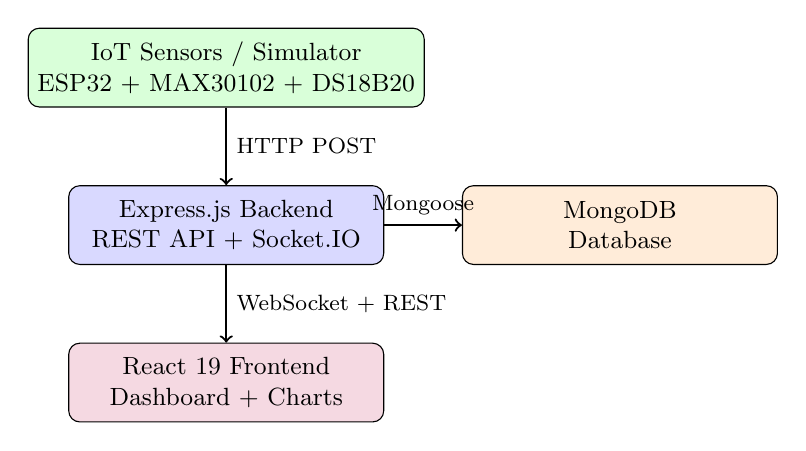
\begin{tikzpicture}[
    box/.style={draw, rounded corners, minimum width=4cm, minimum height=1cm, align=center, font=\small},
    arrow/.style={->, thick}
]
\node[box, fill=green!15] (iot) at (0, 4) {IoT Sensors / Simulator\\ESP32 + MAX30102 + DS18B20};
\node[box, fill=blue!15] (backend) at (0, 2) {Express.js Backend\\REST API + Socket.IO};
\node[box, fill=orange!15] (db) at (5, 2) {MongoDB\\Database};
\node[box, fill=purple!15] (frontend) at (0, 0) {React 19 Frontend\\Dashboard + Charts};

\draw[arrow] (iot) -- node[right, font=\footnotesize] {HTTP POST} (backend);
\draw[arrow] (backend) -- node[above, font=\footnotesize] {Mongoose} (db);
\draw[arrow] (backend) -- node[right, font=\footnotesize] {WebSocket + REST} (frontend);
\end{tikzpicture}
\caption{System Architecture Diagram}
\label{fig:architecture}
\end{figure}

\section{Data Flow}
\begin{enumerate}[leftmargin=*]
    \item \textbf{Data Collection:} IoT sensors (or Python simulator) collect heart rate, SpO2, and temperature readings every 3--5 seconds.
    \item \textbf{Data Transmission:} Readings are sent via HTTP POST to \texttt{/api/health-data} endpoint.
    \item \textbf{Threshold Evaluation:} The \texttt{alertChecker} module evaluates each reading against dual-level thresholds (warning and critical) for all three vitals.
    \item \textbf{Data Persistence:} Valid readings are stored in MongoDB with compound indexing on \texttt{(patientId, timestamp)}.
    \item \textbf{Real-time Broadcast:} Socket.IO emits \texttt{health-data} and \texttt{new-alert} events to all connected clients.
    \item \textbf{Dashboard Update:} React components receive events and update Chart.js graphs with a sliding window of 30 data points.
\end{enumerate}

\section{Authentication \& Authorization}
The system implements a two-layer security model:
\begin{itemize}[leftmargin=*]
    \item \textbf{Authentication (JWT):} On login, the server creates a signed JSON Web Token containing the user ID. The client stores it in localStorage and sends it with every request via the \texttt{Authorization: Bearer} header. The \texttt{auth} middleware verifies the token signature and extracts user identity.
    \item \textbf{Authorization (RBAC):} The \texttt{authorize(...roles)} middleware checks if the requesting user's role is in the permitted roles array. Data-level filtering further restricts query results based on role.
\end{itemize}

\section{Role-Based Data Isolation}
\begin{table}[H]
\centering
\caption{Data Access Matrix by Role}
\label{tab:rbac}
\begin{tabular}{|l|c|c|c|}
\hline
\textbf{Data} & \textbf{Patient} & \textbf{Doctor} & \textbf{Admin} \\
\hline
Patient records & Own only & Assigned only & All \\
\hline
Health data history & Own only & Assigned patients & All \\
\hline
Alerts & Own only & All (can ack) & All (ack + delete) \\
\hline
Reports + AI Analysis & Own upload/view & Upload for assigned & All \\
\hline
User management & --- & --- & Full CRUD \\
\hline
Audit logs & --- & --- & View all \\
\hline
\end{tabular}
\end{table}

\section{Alert Generation Mechanism}
The threshold-based alert engine uses dual-level medical thresholds:
\begin{table}[H]
\centering
\caption{Health Alert Thresholds}
\label{tab:thresholds}
\begin{tabular}{|l|c|c|c|}
\hline
\textbf{Vital Sign} & \textbf{Normal Range} & \textbf{Warning} & \textbf{Critical} \\
\hline
Heart Rate (bpm) & 60--100 & $<$50 or $>$120 & $<$40 or $>$150 \\
\hline
SpO2 (\%) & 95--100 & $<$95 & $<$90 \\
\hline
Temperature (\textdegree C) & 36.1--37.2 & $<$36 or $>$38 & $<$35 or $>$39.5 \\
\hline
\end{tabular}
\end{table}

\section{Patient Registration Workflow}
\begin{enumerate}[leftmargin=*]
    \item Patient self-registers via the login page (restricted to patient role only).
    \item User account is created but \textbf{no Patient medical record} is generated yet.
    \item The patient appears in an ``unlinked users'' pool visible to doctors and admins.
    \item Doctor clicks ``Add Patient'', selects a user, fills clinical details (age, blood group, etc.).
    \item Patient record is created, linked to user account, and assigned to that doctor.
    \item Patient can now log in and see their personalized health dashboard.
\end{enumerate}
